\begin{figure*}[t]
\centering
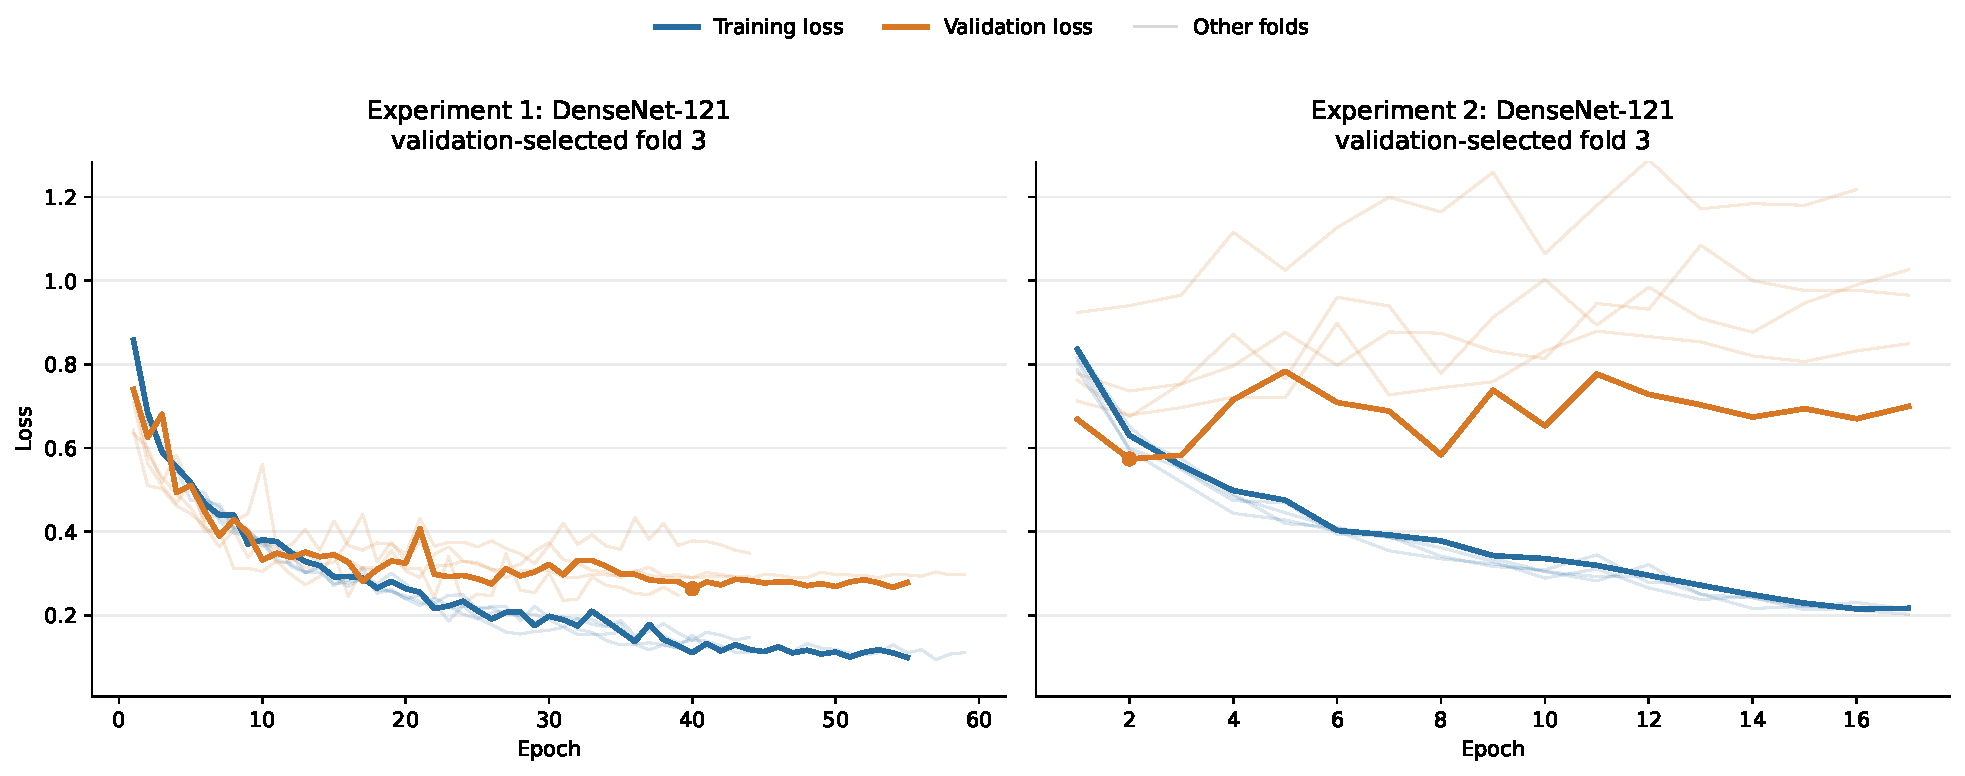
\includegraphics[width=\textwidth]{fig_train_validation_loss.pdf}
\caption{Training and validation loss for the best-performing architecture in each experiment. Lighter lines show all five folds, while darker lines show the fold selected using validation balanced accuracy. The point marks the minimum validation loss of the selected fold.}
\label{fig:train-validation-loss}
\end{figure*}

\begin{figure*}[t]
\centering
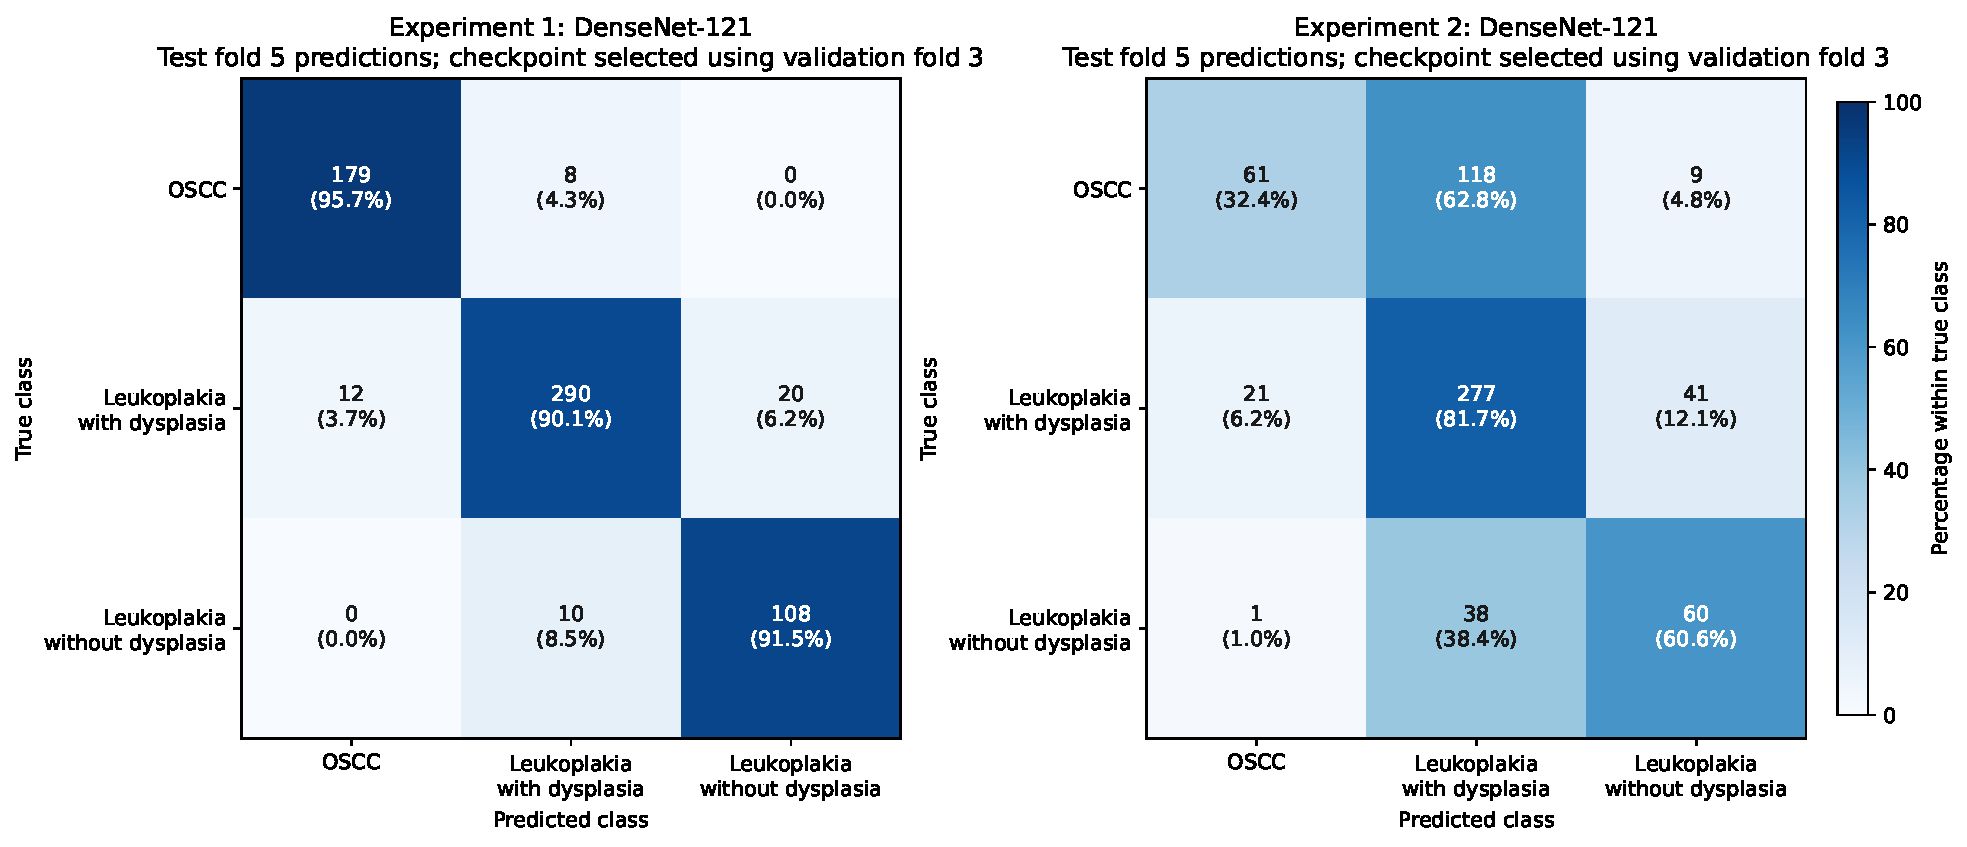
\includegraphics[width=\textwidth]{fig_confusion_matrices.pdf}
\caption{Confusion matrices for test fold 5 in each experiment, using the DenseNet-121 checkpoint selected from validation fold 3. Within DenseNet-121, fold 3 was selected because it had the highest validation balanced accuracy; test fold 5 results were not used to select the representative checkpoint. Cells report counts and percentages within each true class.}
\label{fig:confusion-matrices}
\end{figure*}
